\chapter{Проектирование программного обеспечения} \label{ch:ch2}

\section{Типичные архитектуры Fabric ориентированных приложений} \label{sec:ch2:sec1}
Приложения взаимодействуют с сетью Hyperledger Fabric посредством SDK по протоколу gRPC как показано на рисунке \ref{fig:apps_use_sdk}. 
Они обращаются к узлам бизнес сети для вызова и/или запроса чейнкода, чтения данных из блокчейна, регистрируют слушателей событий, а так же выполня.т различные административные задачи такие как, запрос и/или изменение конфигурации узлов.
\begin{figure}[ht]
	\centering
	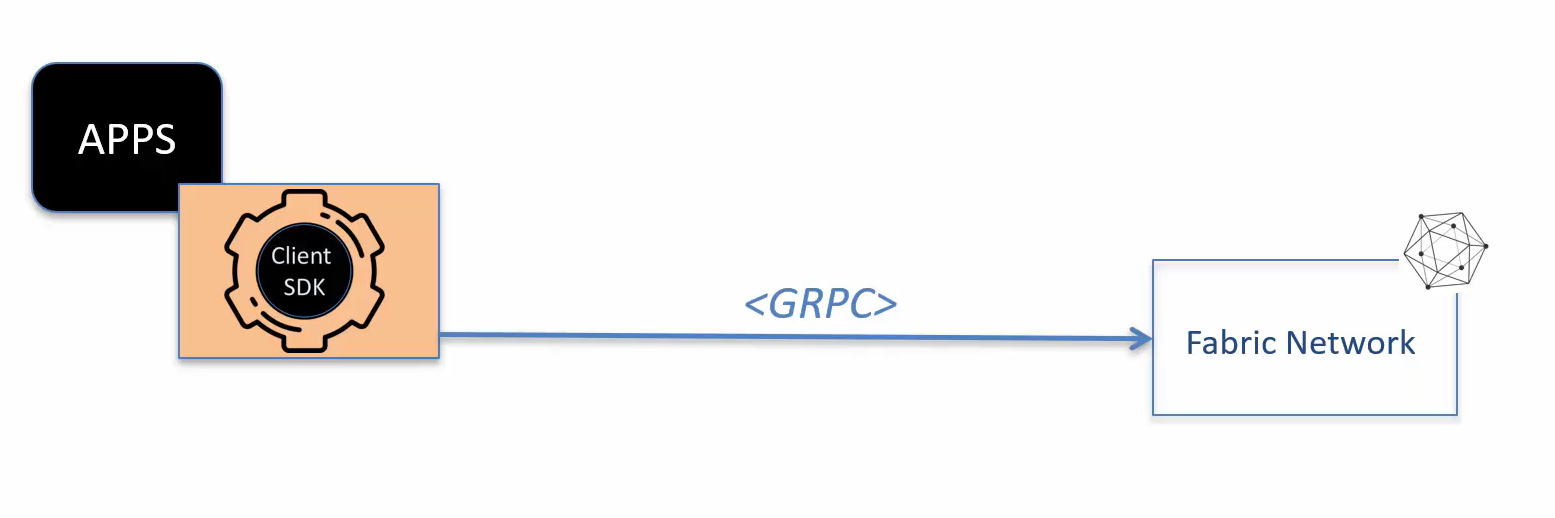
\includegraphics [scale=0.5] {apps_use_sdk}
	\caption{Взаимодействие приложений с Fabric Network}
	\label{fig:apps_use_sdk}
\end{figure}
Как уже упоминалось выше все эти операции осуществляются с помощью Fabric SDK для языков общего назначения. В настоящее время существуют Fabric SDK для языков Java, Go, Python и JavaScript. Так как каждую технологию следует выбирать для тех целей, для которых она подходит лучше всего, то будет справедливым рассмотреть типы Fabric ориентированных приложений. Чаще всего это:
\begin{itemize} 
	\item Графические приложения, позволяющие пользователю выполнять смарт-контракты через графический интерфейс.
	\item Приложения, представляющие отчеты из хранилища данных чейнкода.
	\item Модули интеграции Fabric SDK в уже существующие проекты, для взаимодействия с системами бекенда.
\end{itemize}
При разработки приложения того или иного типа уместно применение соответствующего шаблона архитектуры.
Рассмотрим типичные шаблоны построение Fabric ориентированных приложений.
Настольные приложения - создание и подписание транзакции посходит локально на компьютере пользователя. Такой подход является хорошо защищенным, но имеет недостаток в виде дистрибуции приложения. При внесении правок в приложение, конечный пользователь вынужден в ручную устанавливать обновления на свой компьютер.
\begin{figure}[ht]
	\centering
	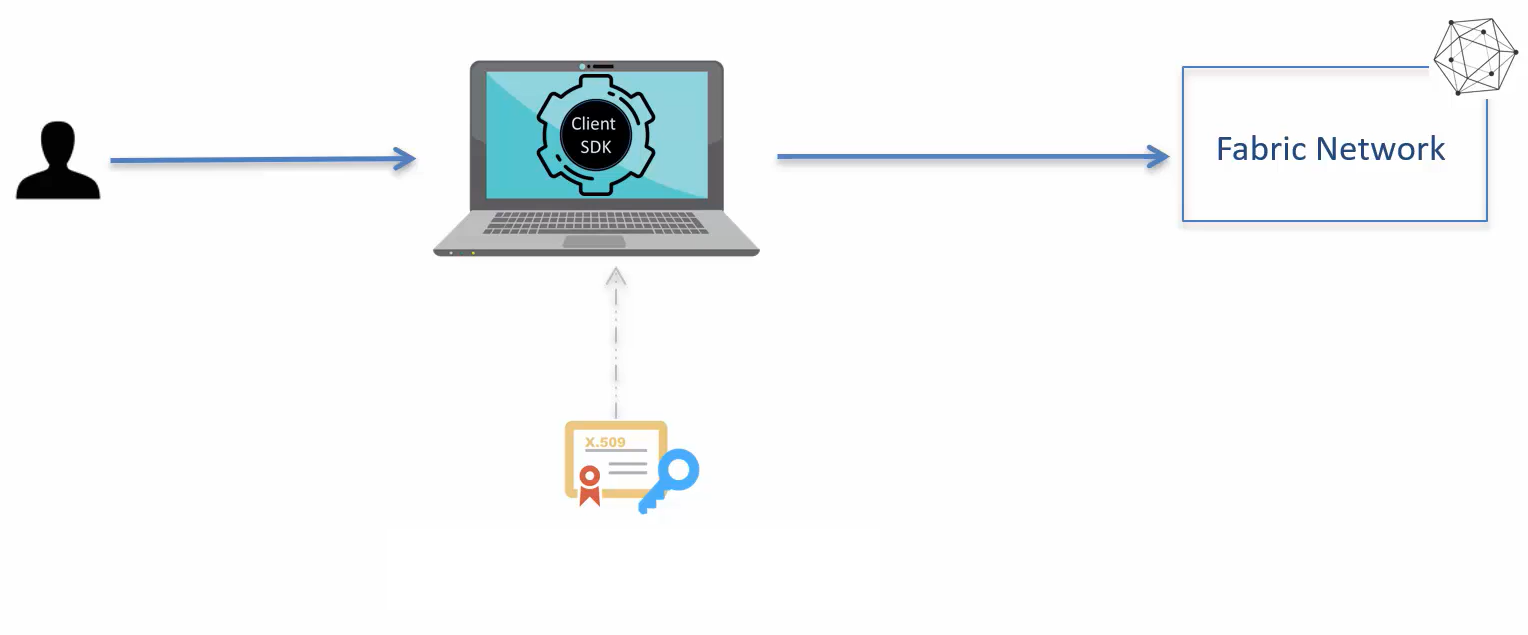
\includegraphics [scale=0.5] {desktop_apps}
	\caption{Настольные приложения, использующие Fabric SDK}
	\label{fig:desktop_apps}
\end{figure}
Обработка транзакций в сети Fabric приводит к возникновению различных событий, которые могут потребляется приложениями. События могут предоставятся клиента посредством некого брокера сообщений (например, Kafka), или же посредством REST-API. При получении определенного события клиентское приложение соответствующим образом обрабатывает его(например, обновляет свои бекенд системы). Так как события инициируются и обрабатываются в режиме реального времени, такой подход широко используется для создания инфопанелей и отчетов в режиме реального времени. Схематично данный шаблон предоставлен на рисунке 
\begin{figure}[ht]
	\centering
	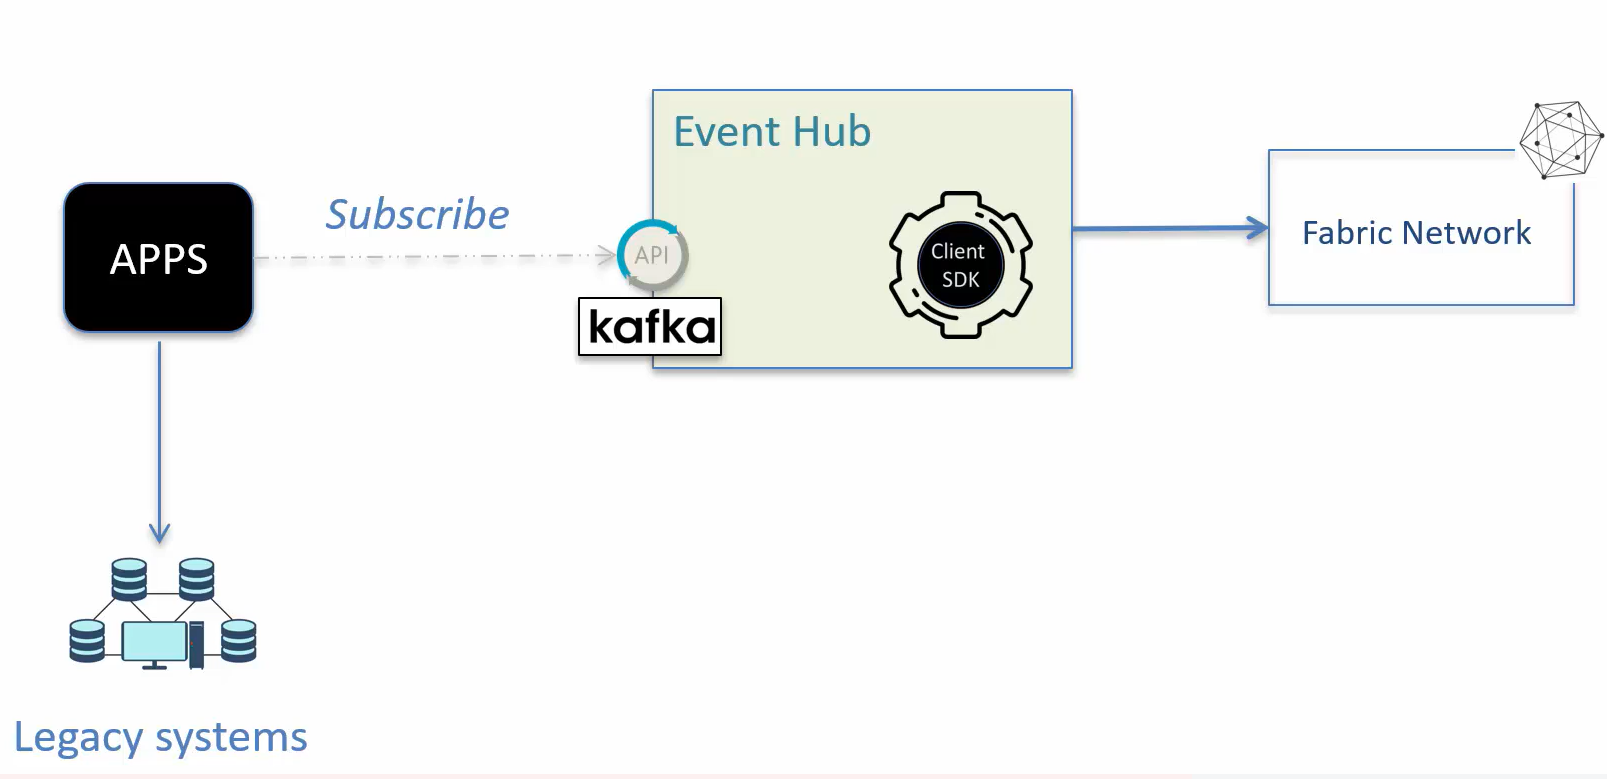
\includegraphics [scale=0.5] {event_hub}
	\caption{Архитектура "Event Hub"}
	\label{fig:event_hub}
\end{figure}
А также Fabric SDK может быть использована для создания различных утилит командной строки. Эти утилиты используется администраторами бизнес сети Hyperledger Fabric для осуществления различных административных задач (Рисунок \ref{fig:admin_cli}).
\begin{figure}[ht]
	\centering
	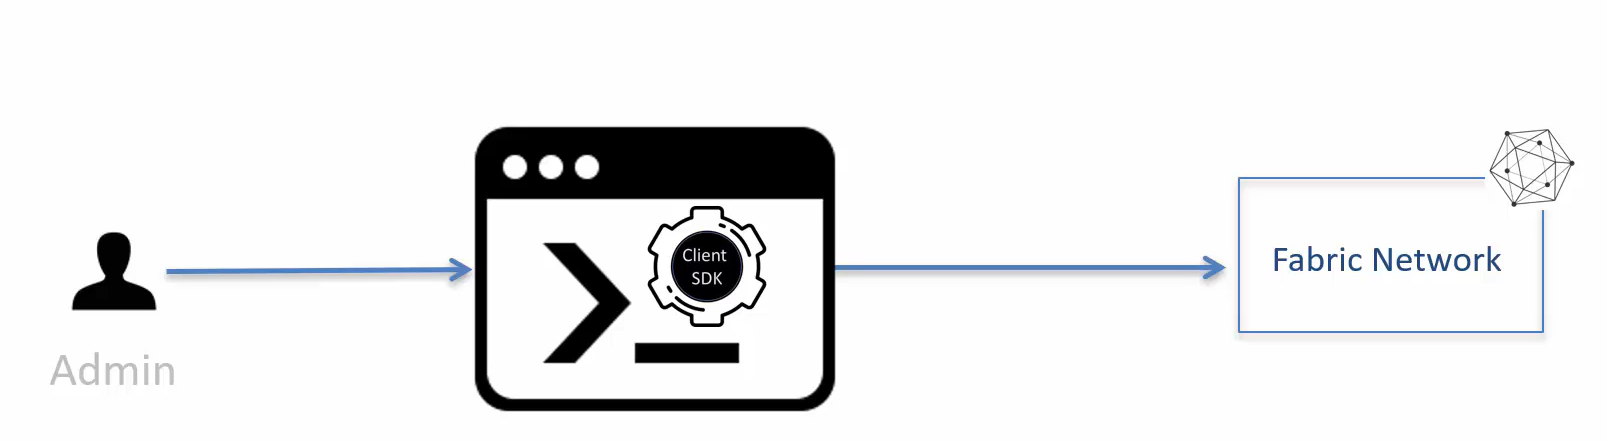
\includegraphics [scale=0.5] {admin_cli}
	\caption{Утилиты командной строки}
	\label{fig:admin_cli}
\end{figure}
Ещё один широк распространенный подход к построению Fabric ориентированных приложений - использование связующего программного обеспечения, ориентированное на обработку сообщений (англ. message-oriented middleware). Это ПО использует Fabric SDK, и обеспечивает связь среды выполнения Fabric с клиентским приложением. Middleware предоставляет API, обращаясь к которому клиентские приложения взаимодействуют с бизнес сетью. При этом тип клиентского приложения может быть любым(настольное, мобильное, веб и д.р.). Cхема такой архитектуры представлена на рисунке
\begin{figure}[ht]
	\centering
	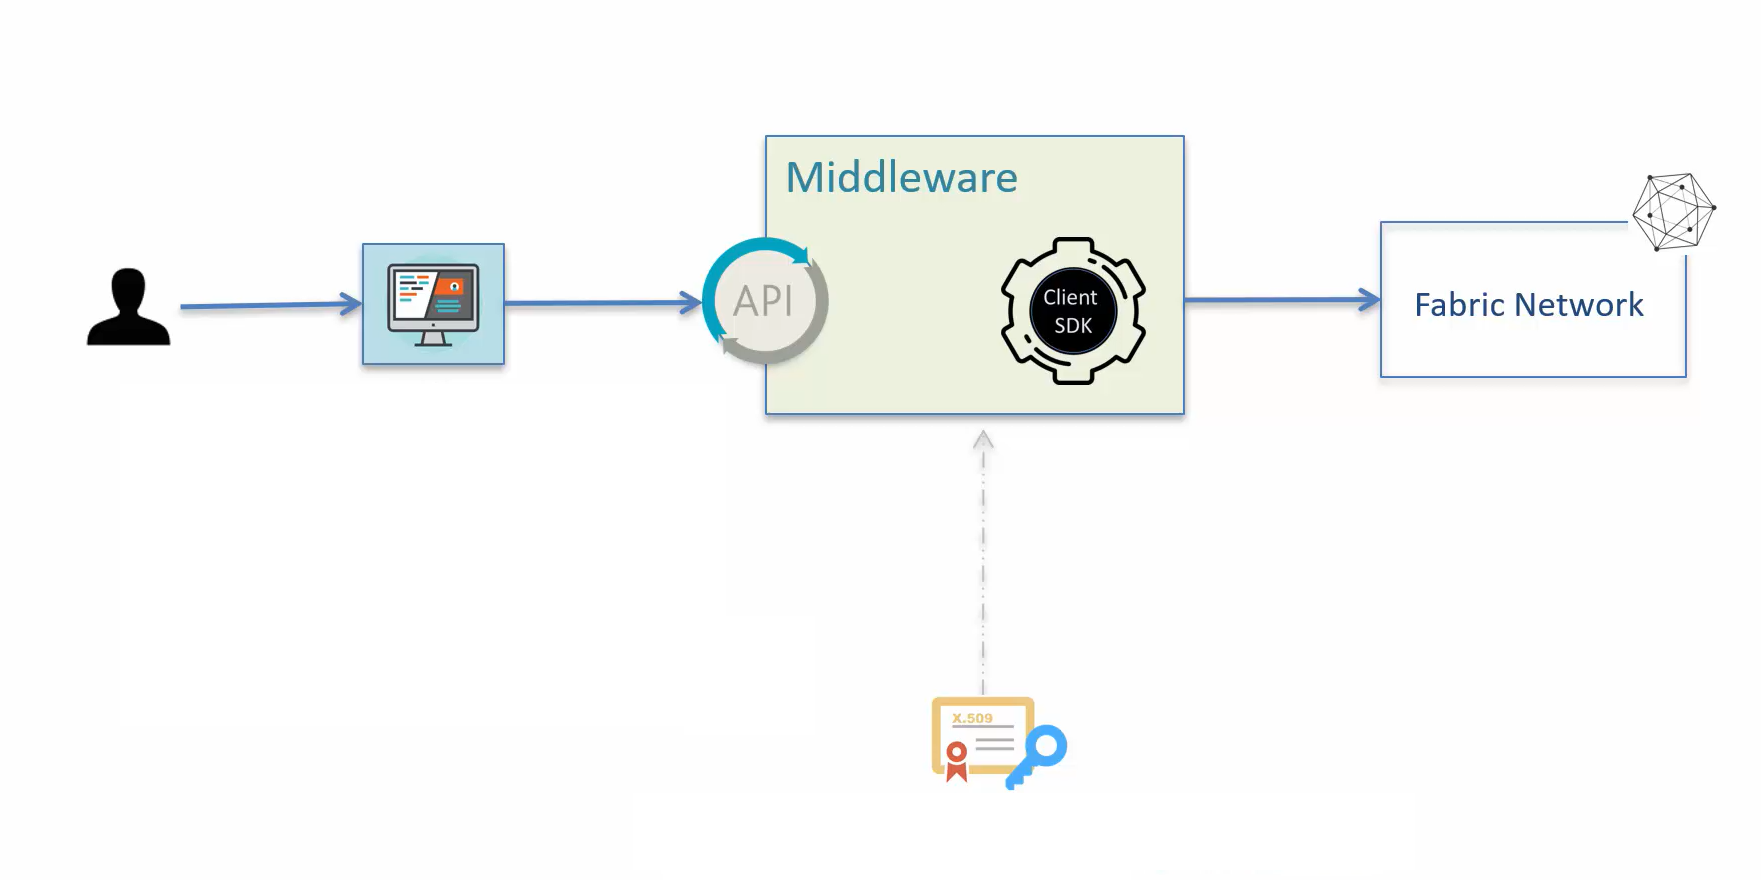
\includegraphics [scale=0.5] {middleware}
	\caption{Архитектура со связующим ПО}
	\label{fig:middleware}
\end{figure}
Но при реализации такого подход возникает ряд вопросов, и первый из них где управлять ключами и сертификатами пользователей? Один из вариантов - управлять ими на стороне middleware. Однако в этом случае пользователи должны доверять хосту middleware, т.к. их приватные ключи оседают на его стороне. Однако в некоторых случаях пользователи могут не доверять организации, осуществляющей хостинг middleware. В таких случаях необходимо закладывать логику работы с приватными ключами и сертификатами на стороне клиентского приложения. Очевидно, что такой подход является более защищенным, однако он так же имеет недостаток в виде увлечения сложности приложения. А также в этом случае нарушается принцип единственной ответственности (SRP). \cite{solid}


	%\section{Обеспечение безопасности REST-сервера} %\label{sec:ch2:sec2}
	%Как миниммум юзать TLS/HTTPs и аутентификацию.

\section{Выбор инструментов и технологий} \label{sec:ch2:sec2}
\subsection{Архитектура} \label{subsec:ch2/sec2/subsec1}
В \ref{sec:ch2:sec1} мы рассмотрели типичные архитектуры  Fabric ориентированных приложений. В данной работе выбор пал на архитектуру со связующим ПО с инкапсуляцией логики работы с сертификатами пользователей на стороне связующего ПО. В представленных в работе сценариях отношение между отдельными элементами доверительные, поэтому недостаток данного подхода не создает проблем. К очевидными плюсам данной архитектуры можно, также отнести легкую замену графического клиентского приложения, т.к. ему неизвестно существование бизнес сети, оно работает исключительно со связующим ПО по технологии RPC. \cite{grpc}
На рисунке \ref{fig:sys_architecture} представлена схема архитектуры разработанного приложения.
\begin{figure}[ht]
	\centering
	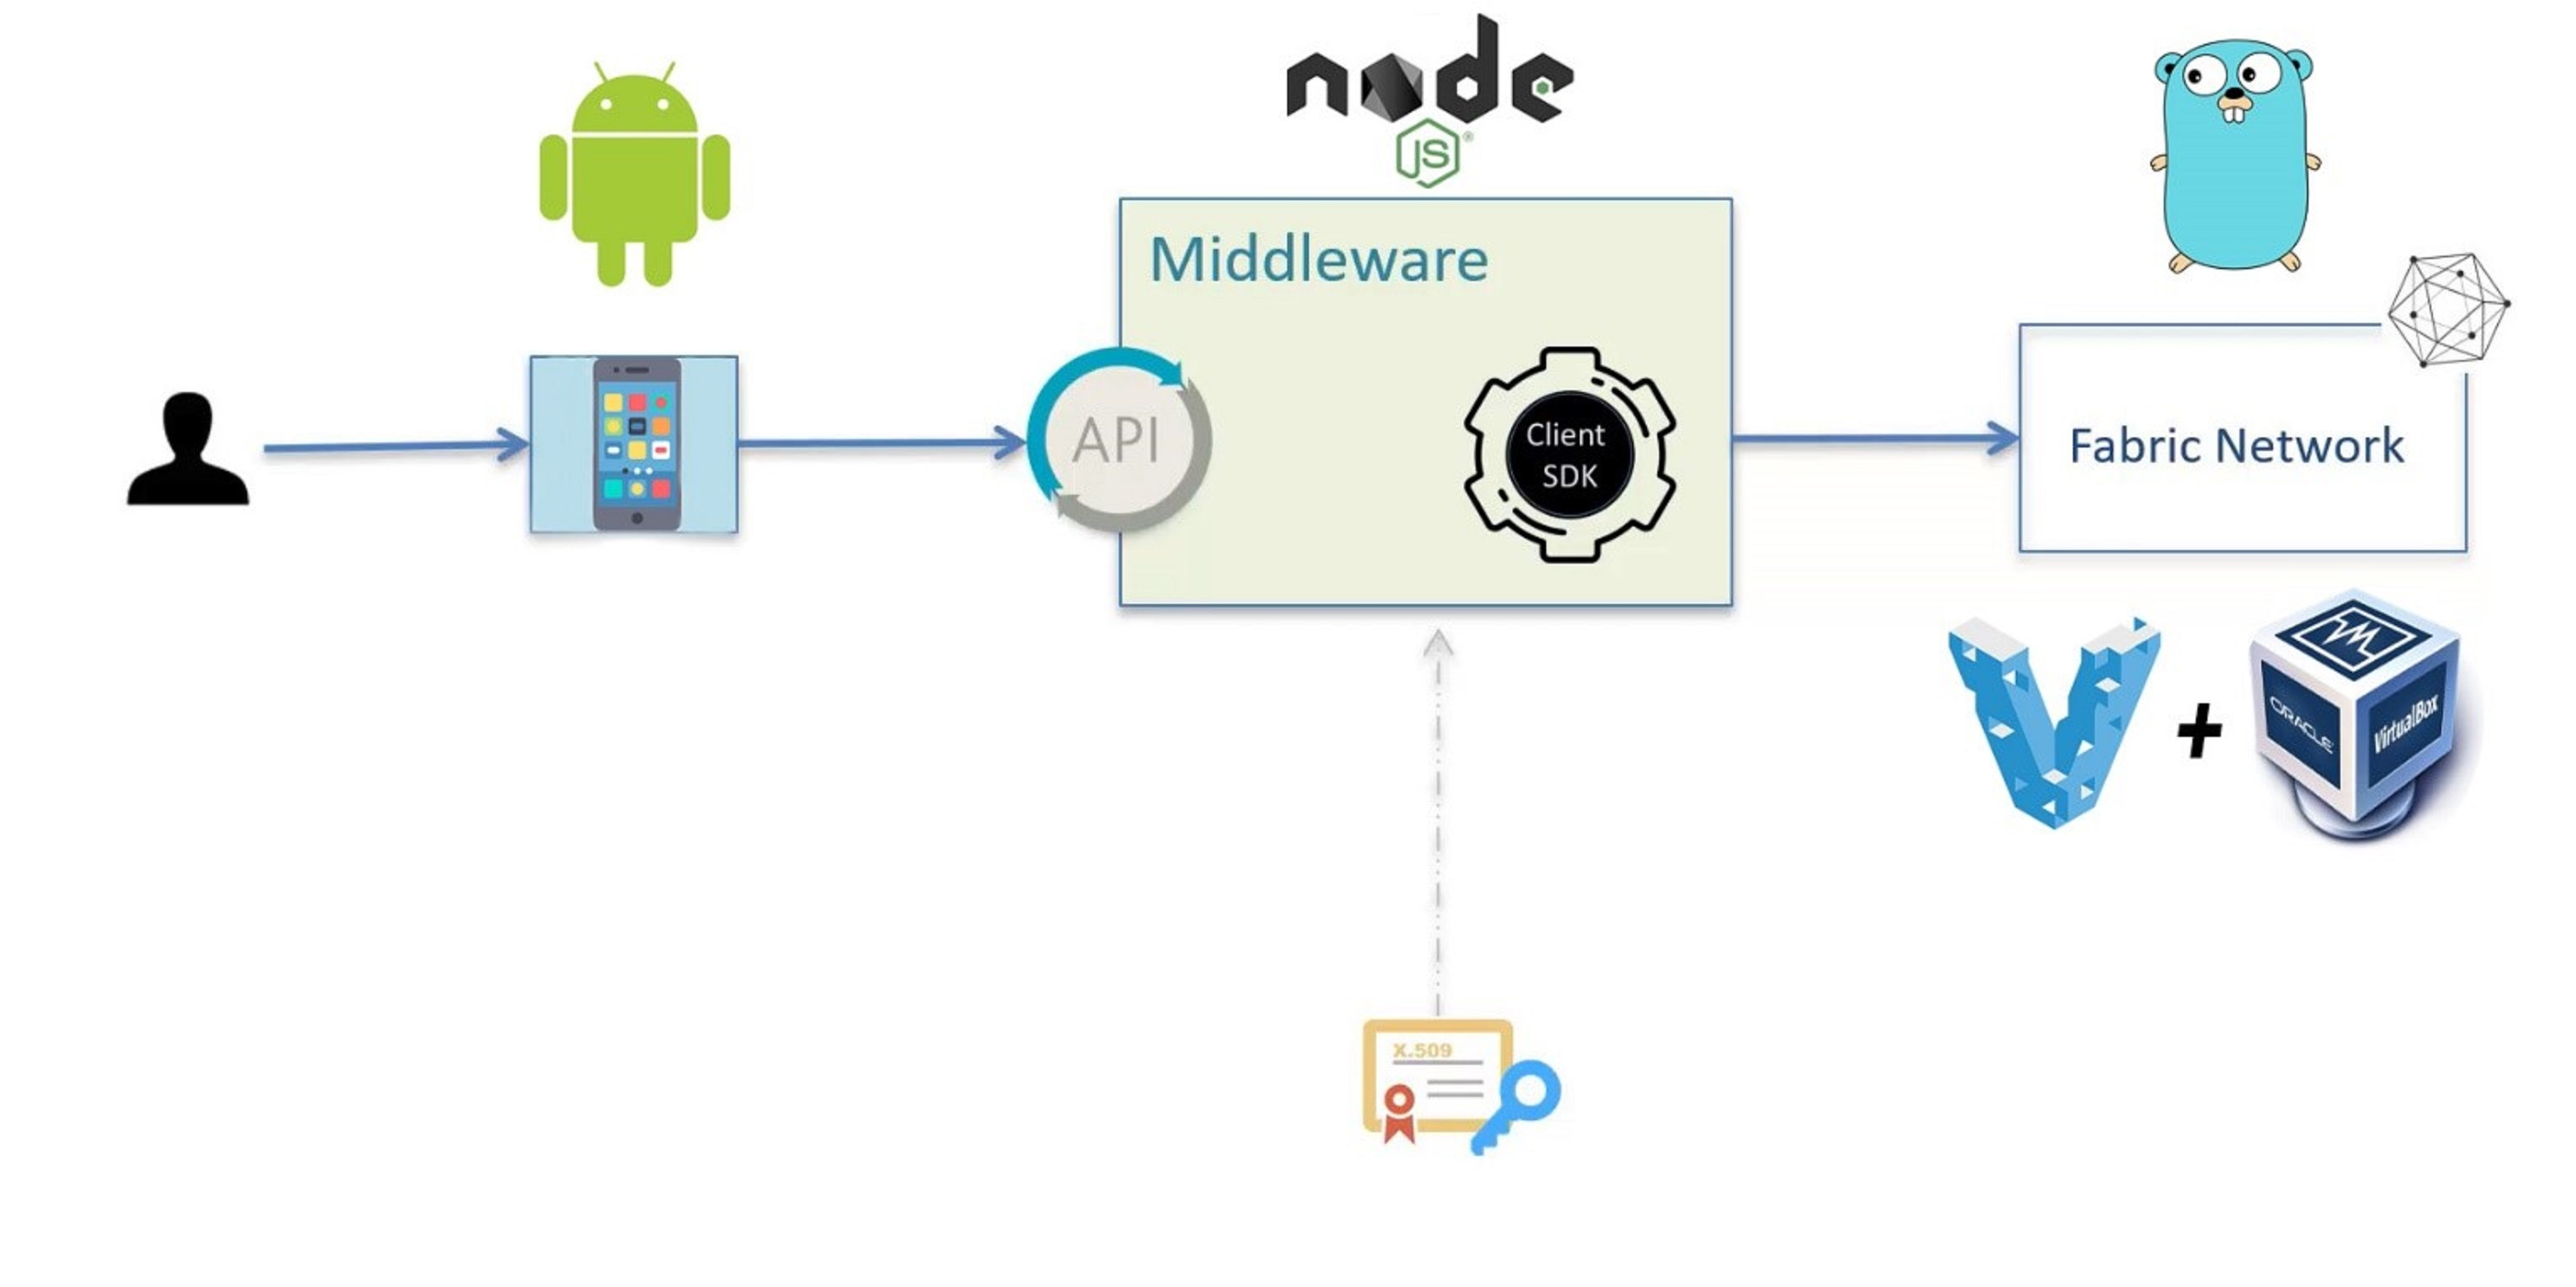
\includegraphics [scale=0.5] {sys_architecture}
	\caption{Архитектура разработанного приложения.}
	\label{fig:sys_architecture}
\end{figure}
Для разработки и отладки смарт контрактов требуется их разворачивание на пирах бизнес сети. Проще всего разворачивать такую тестовую сеть на виртуальной машине, на которую пред установлено  все необходимое программное обеспечение, а именно:
\begin{itemize}
	\item Docker и Docker Compose \cite{docker};
	\item Компилятор и стандартные библиотеки языка Go \cite{golang};
	\item Менеджер пакетов языка Go govendor; 
	\item Бинарные файлы Hyperledger Fabric \cite{fabric-bins};
	\item Пакеты Shim и Shimtest \cite{shim-go}.
\end{itemize}

На это виртуальной машине запускаются docker-контейнеры, представляющие из себя различные элементы бизнес сети Fabric (orderers, endorser, peers). Таким образом, образуются тестовая бизнес сеть внутри которой легко разрабатывать, отлаживать и тестировать смарт контракты. Запуск виртуальной машины и остановка среды разработки происходит с помощью Oracle Virtual Box \cite{oracle-vbox-site} и Vagrant \cite{vagrant-site}.
Отдельно внимания заслуживает такой инструмент как Vagrant, поскольку он сильно облегчает развертку среды разработки. 
Vagrant - это программное обеспечение с открытым исходным кодом, предназначенное для построения и поддержки виртуальных сред разработки на основе, например, Virtual Box, Hyper-V, Docker контейнеров. Основная задача этого инструмента - упростить конфигурационное управление (англ.software configuration management, SCM) \cite{scm} и улучшить продуктивность разработчика. 
Создание виртуальной машины происходит при помощи файла конфигурации Vagrantfile, содержимое которого представлено в листинге \ref{lst:vagrantfile}.

\begin{lstlisting}[caption={Конфигурация виртуальной машины: Vagrantfile},label={lst:vagrantfile},language=Ruby]
	Vagrant.configure("2") do |config|
	config.vm.box = "bento/ubuntu-18.04"
	
	# Проброс портов
	# Для Orderer контейнера
	config.vm.network "forwarded_port", guest: 7050, host: 7050
	# Для Hyperledger Explorer
	config.vm.network "forwarded_port", guest: 8080, host: 8080
	# Для CouchDB
	config.vm.network "forwarded_port", guest: 5984, host: 5984
	
	# Для Peer контейнеров
	config.vm.network "forwarded_port", guest: 7051, host: 7051
	config.vm.network "forwarded_port", guest: 7052, host: 7052
	config.vm.network "forwarded_port", guest: 8051, host: 8051
	config.vm.network "forwarded_port", guest: 8052, host: 8052
	config.vm.network "forwarded_port", guest: 9051, host: 9051
	config.vm.network "forwarded_port", guest: 9052, host: 9052
	config.vm.provision "shell", inline:  $script /home/vagrant/app/sdk/vagrant_node_modules
	end
\end{lstlisting}


После создание виртуальной машины, управление ею осуществляется при помощи выполнения следующих команд в директории с Vagrantfile:
\begin{itemize}
	\item \textit{vagrant up} - запуск машины с заданной конфигурацией;
	\item \textit{vagrant ssh} - подключение к виртуальной машине посредством сетевого протокола SSH;
	\item \textit{vagrant halt} - остановка виртуальной машины;
	\item \textit{vagrant destroy} - удаление виртуальной машины.
\end{itemize}
Таким образом, мы имеем удобную среду для разработки, отладки и тестирования смарт контрактов.

\subsection{Смарт контракты} \label{subsec:ch2/sec2/subsec2}

Написание смарт контрактов осуществляется на языках программирования общего назначения, таких как JavaScript, Java и Go. В данной работы смарт контракты написаны на языке Go - разработанным компанией Google языке со статической типизацией. Синтаксически схож с  языком С, однако имеет преимущества перед ним в виде безопасного доступа к памяти, сборкой мусора и удобством реализации параллельных вычислений.

Смарт контракт на языке Go представляет из себя реализацию интерфейса Chaincode из пакета github.com/hyperledger/fabric-chaincode-go/shim.
 
\begin{lstlisting}[caption={Интерфейс Chaincode},label={lst:ichaincode},language=Go]
 type Chaincode interface {
 	
 	Init(stub ChaincodeStubInterface) pb.Response
 
 	Invoke(stub ChaincodeStubInterface) pb.Response
 	
 }
\end{lstlisting}
 
Как видно из листинга \ref{lst:ichaincode} необходимо реализовать две функции: 

\begin{enumerate}
	\item Init - в ней закладывается логика инициализации внутреннего состояния смарт контракта. Она вызывается в момент создания контейнера смарт контракта.
	\item Invoke - содержит бизнес логику смарт контракта
\end{enumerate}

Помимо этих двух функций необходимо зарегистрировать экземпляр  смарт контракт в среде выполнения Fabric. Кога клиентское приложение обращается к сети Fabric, оно передает ей название смарт контракта, название функции смарт котракта и набор параметров. Среда выполнения сопоставляет переданное название смарт контракта с экземплярами смарт контрактов зарегистрированными в среде выполнения и делегирует обращение клиента соответствующей функции соответствующего смарт контракта. Регистрация смарт контракта осуществляется в главной функции Go (main) посредством вызова функции shim.Start с передачей ей экземпляра смарт контракта в качестве параметра. Таким образом шаблон типичного смарт контракта на языке Go имеет вид представленный в листинге \ref{lst:chaincode-impl}.

\begin{lstlisting}[caption={Реализация Chaincode},label={lst:chaincode-impl},language=Go]
	package main
	
	import (
		"fmt"
		"github.com/hyperledger/fabric-chaincode-go/shim"
		pb "github.com/hyperledger/fabric-protos-go/peer"
	)
	
	// SimpleChaincode - пример смарт контракта
	type SimpleChaincode struct {}

	func (t *SimpleChaincode) Init(stub shim.ChaincodeStubInterface) pb.Response {
		// логика инициализации
	}
	
	func (t *SimpleChaincode) Invoke(stub shim.ChaincodeStubInterface) pb.Response {
		// бизнес логика
	}
	
	func main() {
		err := shim.Start(new(SimpleChaincode))
		if err != nil {
			fmt.Printf("Ошибка регистрации смарт-контракта: %s", err)
		}
	}
\end{lstlisting}


\subsection{REST-сервер} \label{subsec:ch2/sec2/subsec3}
Для обеспечения связи клиентского приложение со связующим ПО в качестве методологии RPC был выбран REST (Representational State Transfer — передача состояния представления)\cite{restful} Философия этого подхода заключается в том, что приложения моделируются как набор ресурсов, с которыми клиенты могут взаимодействовать (считывать данные, обновлять, удалять и т.д.). В наше время построение приложений с помощью архитектурного стиля REST вкупе с HTTP и JSON \cite{js-json} стало фактическим стандартом для создания микросервисов.
Как уже упоминалось в \ref{sec:ch2:sec1}, Fabric SDK существует для нескольких языков программирования общего назначения, среди которых присутствует JavaScript \cite{pure-js}. 
%TODO: Node js \cite{node-js}, npm, express, nodemon \cite{nodemon}

\subsection{Клиентское приложение}
 \label{subsec:ch2/sec2/subsec3}
 
%Т.К. мобильное приложение, а самый распространенная система Андроид то конечно же джава
